\section{Assignment description}
The first assignment of Modelling and Control of Manipulators focuses on the geometric fundamentals and algorithmic tools underlying any robotics application. The concepts of transformation matrix, orientation matrix and the equivalent representations of orientation matrices (Equivalent angle-axis representation and Euler Angles) will be reviewed.

The first assignment is \textbf{mandatory} and consists of 5 different exercises. You are asked to:
\begin{itemize}
    \item Download the .zip file called MCM-LAB1 from the Aulaweb page of this course.
    \item Implement the code to solve the exercises on MATLAB by filling the predefined files called "\textit{main.m}", "\textit{AngleAxisToRot.m}", "\textit{RotToAngleAxis.m}", "\textit{YPRToRot.m}" and "\textit{RotToYPR.m}".
    \item Write a report motivating the answers for each exercise, following the predefind format on this document.
\end{itemize}

\subsection{Exercise 1 - Angle-Axis to Rotation Matrix}
A particularly interesting minimal representation of 3D rotation matrices is the so-called angle-axis representation, where a rotation is represent by the axis of rotation \begin{math}\textbf{h}\end{math} and the angle $\theta$. Any rotation matrix can be represented by its equivalent angle-axis representation by applying the Rodrigues Formula.

%\[ R(^* \textbf{v},\theta) = e^{[^*\textbf{v}\times]\theta} = e^{[\rho\times]} =  \textbf{I}_{3x3} + [^* \textbf{v}\times] \sin(\theta) + [^* \textbf{v}\times]^2 (1-\cos(\theta))\]


\textbf{Q1.1} Given an angle-axis pair \begin{math}(\textbf{h},\theta)\end{math}, implement on MATLAB the Rodrigues formula, computing the equivalent rotation matrix, \textbf{WITHOUT} using built-in matlab functions. The function signature will be


\begin{center}\textit{function R = AngleAxisToRot(h,theta)}\end{center}


Then test it for the following cases and briefly comment the results obtained:
\begin{itemize}
    \item \textbf{Q1.2}\hspace{10mm} \begin{math} \textbf{h} = [1,0,0]^T\end{math} and  \begin{math} \theta = 90^\circ \end{math}
    \item \textbf{Q1.3}\hspace{10mm} \begin{math} \textbf{h} = [0,0,1]^T\end{math} and  \begin{math} \theta = \pi/3 \end{math}
    \item \textbf{Q1.4}\hspace{10mm} \begin{math} \mathbf{\rho} = [-\pi/3, -\pi/6 ,\pi/3];\end{math}
\end{itemize}
\textbf{Note that $\mathbf{\rho} = \textbf{h}\theta$}.
%\subsection{Exercise 2 - Inverse Equivalent Angle-Axis Problem}
\subsection{Exercise 2 - Rotation Matrix to Angle-Axis}
Given a rotation matrix \begin{math}R\end{math}, the problem of finding the corresponding angle-axis representation \begin{math}(\textbf{h},\theta)\end{math} is called the Inverse Equivalent Angle-Axis Problem.
\newline


\textbf{Q2.1} Given a rotation matrix \begin{math}R\end{math}, implement on MATLAB the Equivalent Angle-Axis equations \textbf{WITHOUT} using built-in matlab functions. The function signature will be


\begin{center}\textit{function [h,theta] = RotToAngleAxis(R)}\end{center}


You \textbf{MUST} check that the input is a valid rotation matrix. Test it for the following cases and briefly comment the results obtained:

\begin{itemize}
    \item \textbf{Q2.2}\hspace{10mm} $R = \begin{pmatrix}
        1 & 0 & 0 \\
        0 & 0 & -1 \\
        0 & 1 & 0
    \end{pmatrix}$
    
    \item \textbf{Q2.3}\hspace{10mm} $R = \begin{pmatrix}
        0.5& -\sqrt{3}/2 & 0 \\
        \sqrt{3}/2 & 0.5 & 0 \\
        0 & 0 & 1
    \end{pmatrix}$
    
    \item \textbf{Q2.4}\hspace{10mm} $R = \begin{pmatrix}
        1 & 0 & 0 \\
        0 & 1 & 0 \\
        0 & 0 & 1
    \end{pmatrix}$
    
    \item \textbf{Q2.5}\hspace{10mm} $R = \begin{pmatrix}
        -1 & 0 & 0 \\
        0 & -1 & 0 \\
        0 & 0 & 1
    \end{pmatrix}$
\end{itemize}

\subsection{Exercise 3 - Euler Angles to Rotation Matrix}
Any orientation matrix can be expressed in terms of three elementary rotations in sequence. Consider the Yaw Pitch Roll (YPR) representation, where the sequence of the rotation axes is Z-Y-X.
\newline

\textbf{Q3.1} Given a triplet of YPR angles ($\psi$, $\theta$, $\phi$), compute the equivalent rotation matrix representation \textbf{WITHOUT} using built-in matlab functions. The function signature will be


\begin{center}\textit{function R = YPRToRot(psi, theta, phi)}\end{center}


Then test it for the following cases and briefly comment the results obtained:


\begin{itemize}
    \item \textbf{Q3.2}\hspace{10mm} $\psi=\theta=0$, $\phi=\pi/2$
    \item \textbf{Q3.3}\hspace{10mm} $\phi=\theta=0$, $\psi=60^\circ$
    \item \textbf{Q3.4}\hspace{10mm} $\psi=\pi/3$, $\theta=\pi/2$, $\phi=\pi/4$
    \item \textbf{Q3.5}\hspace{10mm} $\psi=0$, $\theta=\pi/2$, $\phi=-\pi/12$
\end{itemize}

\subsection{Exercise 4 - Rotation Matrix to Euler Angles}
Given a rotation matrix \begin{math}R\end{math}, it is possible to compute an equivalent triplet of YPR angles ($\psi$, $\theta$, $\phi$), provided that the configuration is not singular (that is, $\cos{\theta} \ne 0$).
\newline

\textbf{Q4.1} Given a rotation matrix \begin{math}R\end{math}, implement in MATLAB the equivalent YPR angles, \textbf{WITHOUT} using built-in matlab functions. The function signature will be


\begin{center}\textit{function [psi,theta,phi] = rotToYPR(R)}\end{center}


You \textbf{MUST} check that the input is a valid rotation matrix. Test it for the following cases and briefly comment the results obtained:


\begin{itemize}
    \item $\textbf{Q4.2}\hspace{10mm} R = \begin{pmatrix}
        1 & 0 & 0 \\
        0 & 0 & -1 \\
        0 & 1 & 0
    \end{pmatrix}$
    
    \item $\textbf{Q4.3}\hspace{10mm} R = \begin{pmatrix}
        \frac{1}{2} & -\frac{\sqrt{3}}{2} & 0 \\
        \frac{\sqrt{3}}{2} & \frac{1}{2} & 0 \\
        0 & 0 & 1
    \end{pmatrix}$
    
    \item $\textbf{Q4.4}\hspace{10mm} R = \begin{pmatrix}
        0 & -\frac{\sqrt{2}}{2} & \frac{\sqrt{2}}{2} \\
        0.5 & \frac{\sqrt{2}\sqrt{3}}{4} & \frac{\sqrt{2}\sqrt{3}}{4} \\
        -\frac{\sqrt{3}}{2} & \frac{\sqrt{2}}{4} & \frac{\sqrt{2}}{4}
    \end{pmatrix}$
\end{itemize}

\subsection{Exercise 5 - Frame tree}

\begin{figure}
\centering
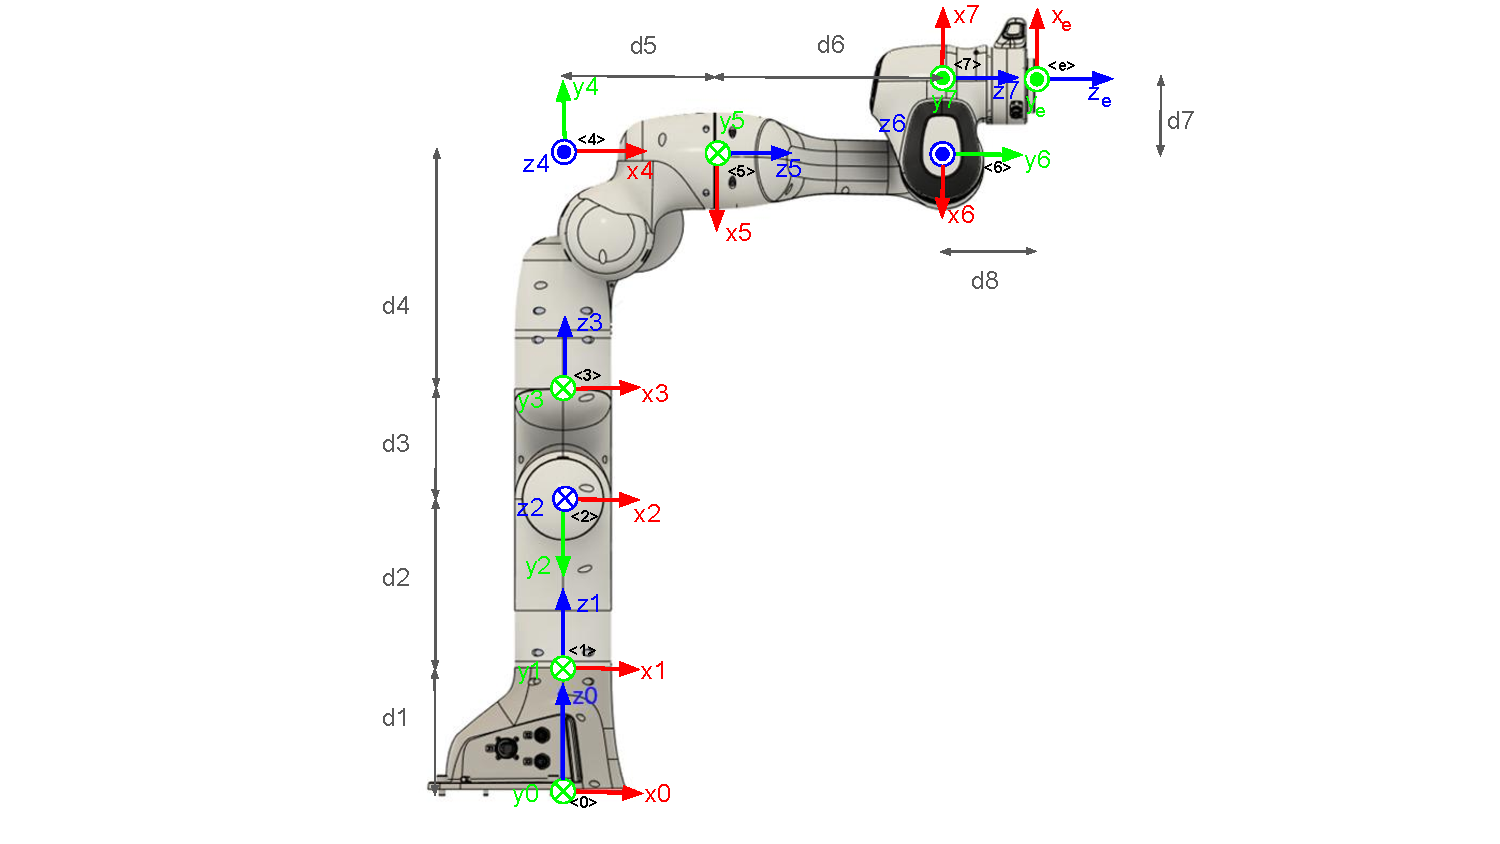
\includegraphics[width=1\linewidth]{Resources/franka.pdf}
\caption{exercise 5 frames}
\label{fig:ex2}
\end{figure}

Figure \ref{fig:ex2} shows the frame tree for the 7 joints of the Franka robot. With reference to the figure, use the geometric definition of the transformation matrix to compute by hand the following matrices.
\begin{itemize}
\item \textbf{Q5.1} \hspace{10mm} $^0_1 T$
\item \textbf{Q5.2} \hspace{10mm} $^1_2 T$
\item \textbf{Q5.3} \hspace{10mm} $^2_3 T$
\item \textbf{Q5.4} \hspace{10mm} $^3_4 T$
\item \textbf{Q5.5} \hspace{10mm} $^4_5 T$
\item \textbf{Q5.6} \hspace{10mm} $^5_6 T$
\item \textbf{Q5.7} \hspace{10mm} $^6_7 T$
\item \textbf{Q5.8} \hspace{10mm} $^7_e T$
\end{itemize}

You \textbf{MUST} compute the matrices \textbf{WITHOUT} using mathematical software.

\newpage
